%250
\documentclass[a4paper,14pt]{extreport}
\usepackage[left=1.5cm,right=1.5cm,
    top=1.5cm,bottom=2cm,bindingoffset=0cm]{geometry}
\usepackage{scrextend}
\usepackage[T1,T2A]{fontenc}
\usepackage[utf8]{inputenc}
\usepackage[english,russian,ukrainian]{babel}
\usepackage{tabularx}
\usepackage{amssymb}
\usepackage{color}
\usepackage{amsmath}
\usepackage{mathrsfs}
\usepackage{listings}
\usepackage{graphicx}
\graphicspath{ {./images/} }
\usepackage{lipsum}
\usepackage{xcolor}
\usepackage{hyperref}
\usepackage{tcolorbox}
\usepackage{tikz}
\usepackage[framemethod=TikZ]{mdframed}
\usepackage{wrapfig,boxedminipage,lipsum}
\mdfdefinestyle{MyFrame}{%
linecolor=blue,outerlinewidth=2pt,roundcorner=20pt,innertopmargin=\baselineskip,innerbottommargin=\baselineskip,innerrightmargin=20pt,innerleftmargin=20pt,backgroundcolor=gray!50!white}
 \usepackage{csvsimple}
 \usepackage{supertabular}
\usepackage{pdflscape}
\usepackage{fancyvrb}
%\usepackage{comment}
\usepackage{array,tabularx}
\usepackage{colortbl}
\usepackage{fp}

\usepackage{varwidth}
\tcbuselibrary{skins}
\usepackage{fancybox}


\usepackage{tikz}
\usepackage[framemethod=TikZ]{mdframed}
\usepackage{xcolor}
\usetikzlibrary{calc}
\makeatletter
\newlength{\mylength}
\xdef\CircleFactor{1.1}
\setlength\mylength{\dimexpr\f@size pt}
\newsavebox{\mybox}
\newcommand*\circled[2][draw=blue]{\savebox\mybox{\vbox{\vphantom{WL1/}#1}}\setlength\mylength{\dimexpr\CircleFactor\dimexpr\ht\mybox+\dp\mybox\relax\relax}\tikzset{mystyle/.style={circle,#1,minimum height={\mylength}}}
\tikz[baseline=(char.base)]
\node[mystyle] (char) {#2};}
\makeatother

\definecolor{ggreen}{rgb}{0.4,1,0}
\definecolor{rred}{rgb}{1,0.1,0.1}
\definecolor{amber}{rgb}{1.0, 0.75, 0.0}
\definecolor{babyblue}{rgb}{0.54, 0.81, 0.94}
\definecolor{amethyst}{rgb}{0.6, 0.4, 0.8}

\usepackage{float}
\usepackage{wrapfig}
\usepackage{framed}
%for nice Code{
\lstdefinestyle{customc}{
  belowcaptionskip=1\baselineskip,
  breaklines=true,
  frame=L,
  xleftmargin=\parindent,
  language=C,
  showstringspaces=false,
  basicstyle=\small\ttfamily,
  keywordstyle=\bfseries\color{green!40!black},
  commentstyle=\itshape\color{purple!40!black},
  identifierstyle=\color{blue},
  stringstyle=\color{orange},
}
\lstset{escapechar=@,style=customc}
%}


\begin{document}
\pagecolor{white}

%----------------------------------------1
\newtcbox{\xmybox}[1][red]{on line, arc=7pt,colback=#1!10!white,colframe=#1!50!black, before upper={\rule[-3pt]{0pt}{10pt}},boxrule=1pt, boxsep=0pt,left=6pt,right=6pt,top=2pt,bottom=2pt}



\begin{titlepage}
  \begin{center}
    \large
    Національний технічний університет України \\ "Київський політехнічний інститут імені Ігоря Сікорського"


    Факультет Електроніки

    Кафедра мікроелектроніки
    \vfill

    \textsc{ЗВІТ}\\

    {\Large Про виконання лабораторної роботи №6\\
      з дисципліни: «Твердотільна електроніки-2»\\[1cm]

      «ІНТЕГРАЛЬНІ СХЕМИ СТАТИЧНОЇ ЛОГІКИ НА МДН – ТРАНЗИСТОРАХ» \\

    }
  \bigskip
\end{center}
\vfill

\newlength{\ML}
\settowidth{\ML}{«\underline{\hspace{0.4cm}}» \underline{\hspace{2cm}}}
\hfill
\begin{minipage}{1\textwidth}
Виконавець:\\
Студент 3-го курсу \hspace{4cm} $\underset{\text{(підпис)}}{\underline{\hspace{0.2\textwidth}}}$  \hspace{1cm}О.\,О.Грабар\\
\vspace{1cm}

Превірив: \hspace{6.1cm} $\underset{\text{(підпис)}}{\underline{\hspace{0.2\textwidth}}}$  \hspace{1cm}Л.\,М.~Королевич\\

\end{minipage}

\vfill

\begin{center}
2021
\end{center}
\end{titlepage}
%---------------------------------------------------------------------------------------------------------------------------------------------------------------------------------



\begin{center}1. МЕТА РОБОТИ\\ \end{center}

Дослідження характеристик керуючого транзистора та властивостей
базових інверторів інтегральних схем виготовлених за МДН-технологією.

\begin{center}2. ЗАВДАННЯ\\ \end{center}

2.1 Виконати вимірювання сімейства вихідних вольт-амперних характеристик керуючого інтегрального МДН-транзистора $T_{y}-$ залежності струму стоку від напруги сток-виток. Побудувати сімейство характеристик $I_{c}=I_{c}\left(U_{c c}\right)[$ при $\left.U_{3}=\mathrm{const}\right]$ на одному малюнку.\\

2.2 Визначити крутизну, динамічний опір стоку, коефіцієнт підсилення напруги
- для крутої і для пологої областей вихідних характеристик транзистора $\left(S_{1} ;\right.$ $\left.S_{2} ; r_{c_l} ; r_{c_2} ; \mu_{1} ; \mu_{2}\right)$\\

2.3 Виміряти передавальні характеристики інтегрального МДН-інвертора при різних $\quad$ видах навантаження: а) лінійний резистор $R_{n}$, б) МДН-транзистор $T_{y}$ ідентичний керуючому, в) МДН-транзистор з довгим та вузьким каналом $T_{n} .$\\

2.4 Побудувати на одному малюнку графіки передавальних характеристик Знятих $\quad$ для $\quad$ трьох типів інверторів. Визначити коефіцієнти передачі для різних видів навантажень.\\

2.5 За результатами вимірювань побудувати на сімействі вихідних ВАХ керуючого транзистора навантажувальні характеристики для трьох типів навантаження: $R_{n}, T_{y}, T_{n}$\\


2.6 Виконати порівняльний аналіз досліджуваних схем інверторів і зробити висновки про доцільність використання розглянутих типів навантаження в схемах статичної логіки.\\

2.7 Намалюйте можливу структуру одного із досліджених інтегральних МДНінверторів (найоптимальнішого). Запропонуйте заходи щодо зниження порогової напруги та зменшення паразитних ємностей інтегрального МДН інвертора.\\



\newpage

\begin{figure}[h]
\center{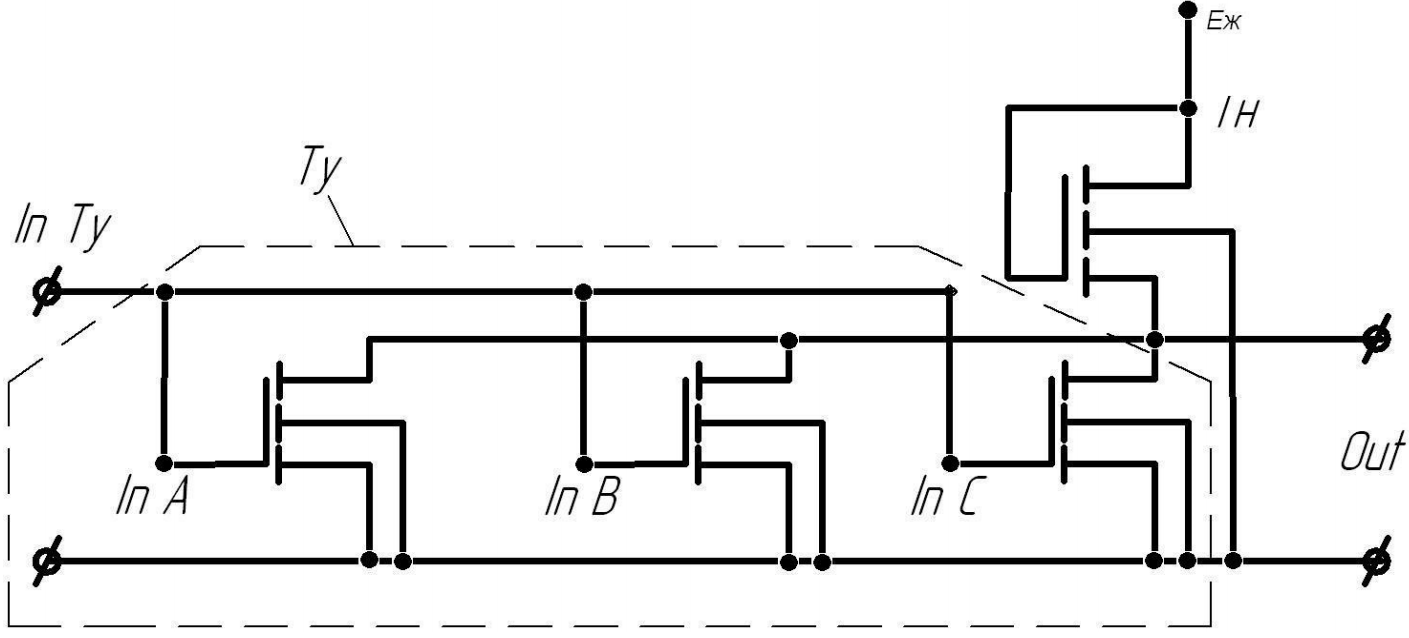
\includegraphics[width=0.8\linewidth]{1.png}}
\caption{Еквівалентна схема $Т_y$ з каналом $W_{\text{экв.}}=3W$.}
\label{ris1}
\end{figure}

\begin{figure}[h]
\center{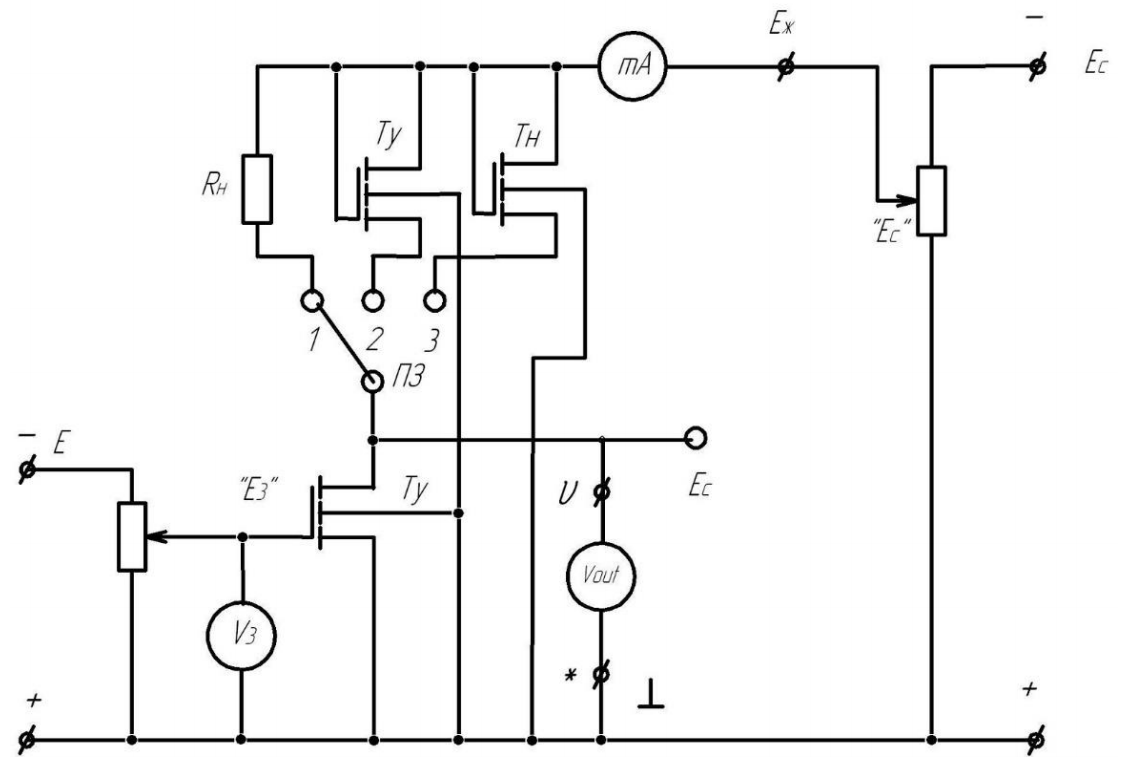
\includegraphics[width=0.8\linewidth]{2.png}}
\caption{Схема дослідження.}
\label{ris2}
\end{figure}




%---------------------------------------------------------------------------------------------------------------------------------------------------------------------------------
\newpage
\begin{figure}[h]
Таб. 1: Сімейство вихідних характеристик керуючого МДН-транзистора.
\center{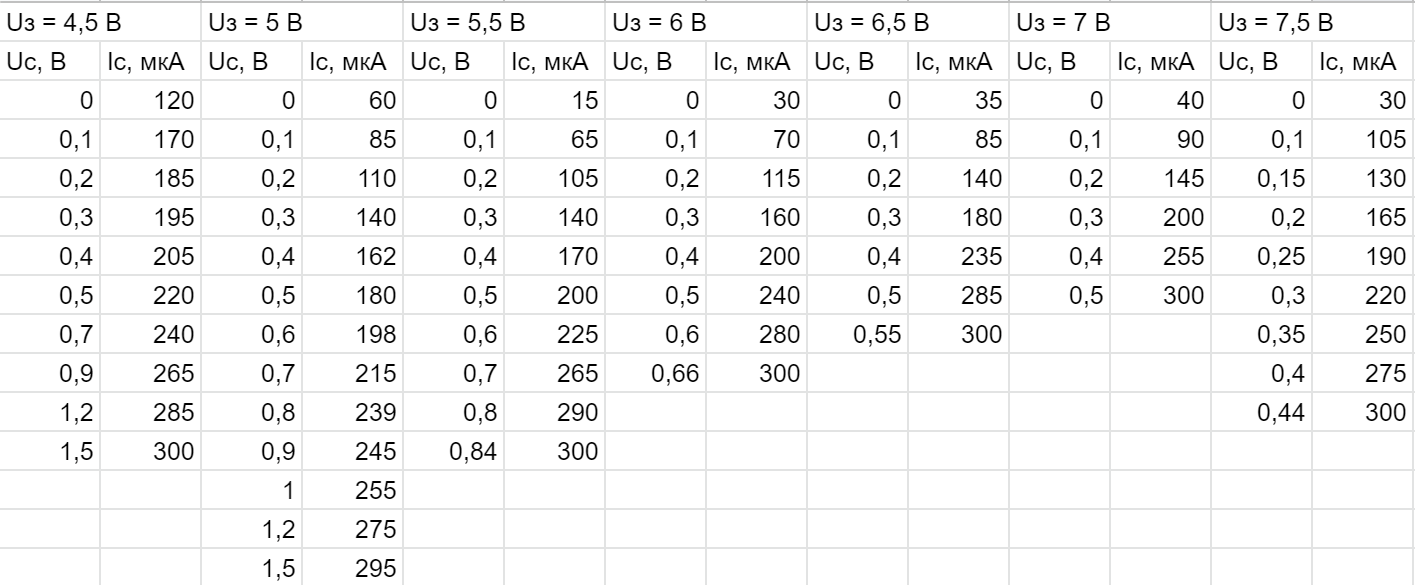
\includegraphics[width=0.9\linewidth]{3.png}}
\label{ris2}
\end{figure}

\vspace{1cm}

\begin{figure}[h]
Таб. 2: Передавальні характеристики МДН інтегрального інвертора для різних видів навантажень.
\center{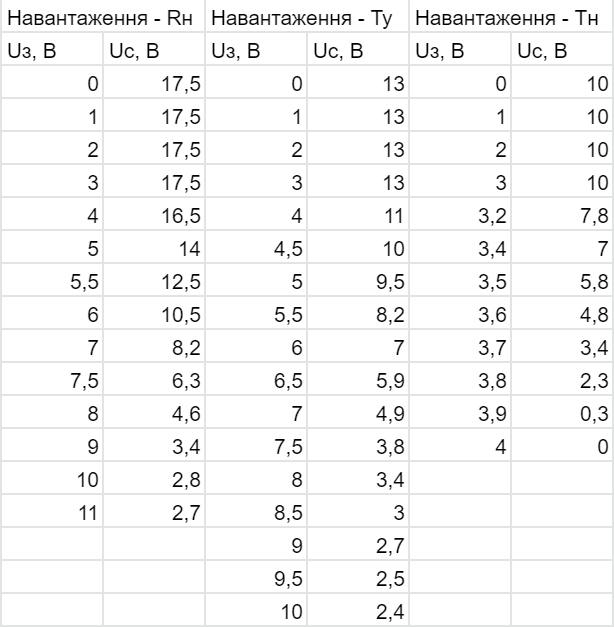
\includegraphics[width=0.55\linewidth]{4.png}}
\end{figure}
\clearpage


\newpage
\begin{center}2. ВИКОНАННЯ РОБОТИ\\ \end{center}

  \begin{figure}[h]
  \center{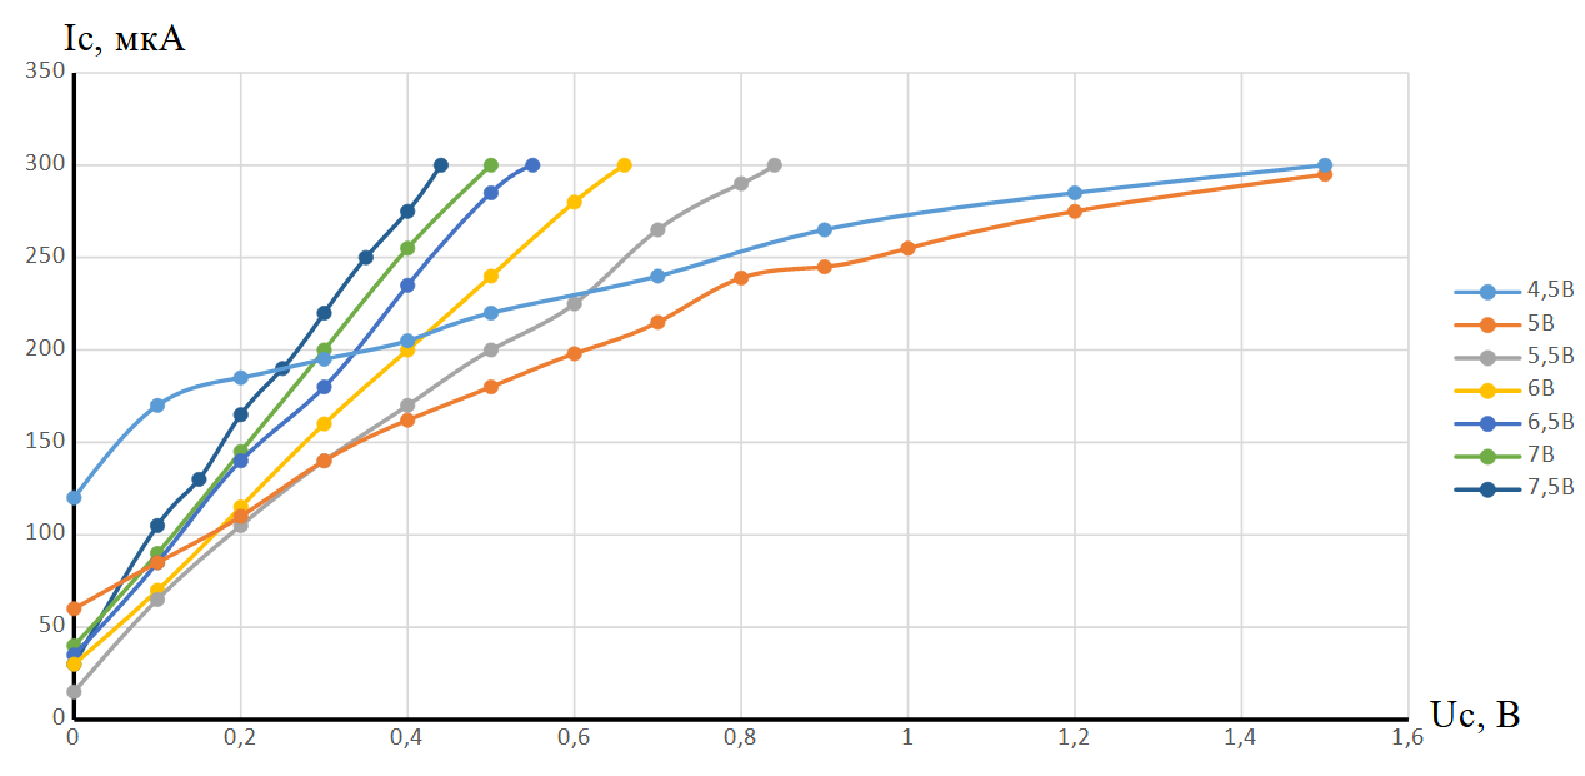
\includegraphics[width=0.9\linewidth]{5.pdf}}
  \caption{Вихідні характеристики транзистора}
  \end{figure}

\vspace{1cm}


\begin{figure}[h]
\center{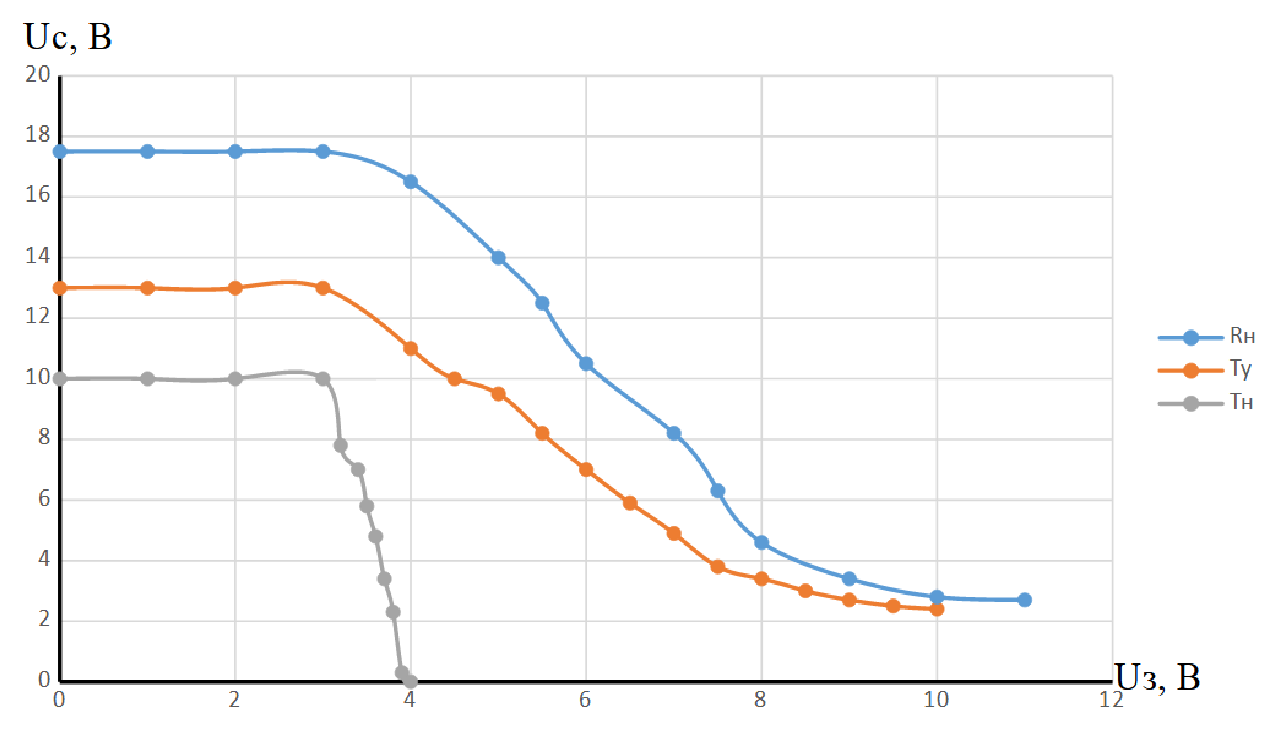
\includegraphics[width=0.85\linewidth]{6.pdf}}
\caption{Передавальні характеристики для трьох типів інверторів}
\end{figure}


\newpage

\FPeval\s{round( (((236-200)*10^{-6})/0.5):8 )}

Можна знайти  крутизну характеристики при $\triangle U_{\text{СВ}} = const$:
\begin{align*}
  S = \dfrac{\triangle I_C}{\triangle U_{\text{3}}} =  \dfrac{(236-200)\cdot10^{-6}}{0,5} = 72 \text{ } \dfrac{\text{ мкА}}{B}
\end{align*}

Тепер можна знайти диференційний опір при $\triangle U_{\text{З}} = const$:
\FPeval\ri{round((0.38/(30*10^{-6})):2) }
\begin{align*}
  r_i = \dfrac{\triangle U_{BC}}{\triangle I_{C_2}} = \dfrac{0.29}{30\cdot 10^{-6}} =  12,6\text{ кОм}
\end{align*}

І тепер можна занати граничний кофіцієнт підсилення за напругою:
\FPeval\ku{round( ( s*ri ):2 )}
\begin{align*}
 K_U = S\cdot r_i = S\cdot r_i =  0,91
\end{align*}











Тепер за формулою $K = \dfrac{\triangle U_C}{\triangle U_3}$ та знаходимо:\\

Для Tн
\FPeval\a{6-4}

\FPeval\tn{round(a/(3.82-3.34):1)}
\begin{align*}
  K_{Tn} = \dfrac{6-4}{3,82-3,74} \approx \FPprint{tn}
\end{align*}

Для Tу
\FPeval\ty{round(a/(7.67-6.43):1)}
\begin{align*}
  K_{Ty} = \dfrac{6-4}{7,67-6,43} \approx \FPprint{ty}
\end{align*}

Для Rн
\FPeval\rn{round(a/(8.45-6.66):1)}
\begin{align*}
  K_{Rn} = \dfrac{6-4}{8,45-6,66} \approx \FPprint{rn}
\end{align*}



\newpage
\begin{figure}[h]
\center{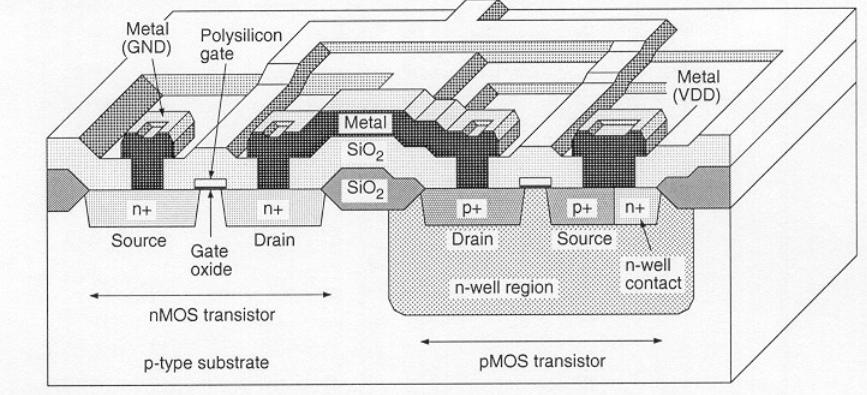
\includegraphics[width=0.8\linewidth]{1.jpg}}
\caption{ Одна з оптимальних cтруктур КМОП iнвертора}
\end{figure}

%\noindent{\color{red} \rule{\linewidth}{1mm} }


\begin{center}
 \textbf{Висновок}
\end{center}

У цій лабораторній роботі було побудовано сімейство вихідних вольт-амперних характеристик керуючого інтегрального МДН-транзистора.  На сімействах вихідних характеристик 
гарно помітна лінійна область зміни, та зона насичення, можна сказати, що отриманi на практицi ВАХ
вiдповiдають теоретичним припущенням, оскильки на всiх сiмействах добре вихідна дилянка змини, а перехiдні характеристики спадають,
починаючи зi значення очевидного занченя
Наступним кроком визначили крутизну, динамiчний опiр стоку, коефiцiєнт пiдсилення напруги для крутої області вихiдних характеристик транзистора, а от для поллогої ми не можемо -- у нас немає вимірів для пологої частини ВАХ, за побудованими на малюнку графiками передавальних характеристик знятих для трьох типiв iнверторiв визначили К для $R_{n}, T_{y} $ та  $ T_{n}$.










\end{document}
